\newpage
\section{Les programmes en Europe : introduction}
\newthought{Nous l'avons vu,} les agences américaines sont assez prolifiques en
matière de programmes de surveillance (avec un budget estimé à 10.3 milliards de
dollars pour la NSA\autocite{budget}, en même temps\ldots), mais nous allons voir
que les pays européens ne sont pas en reste, avec notamment trois grands compétiteurs sur ce
créneau, le Royaume-Uni, l'Allemagne, et la France.

\section{Le Royaume-Uni et le GCHQ}

\newthought{C'est LE champion} européen de la surveillance électronique de
masse. Le Royaume-Uni a une longue tradition dans le domaine du chiffre, il
n'est donc pas surprenant de voir les Britanniques très en avance dans ce
domaine. Leur partenariat historique avec les \EUA~en font les acteurs
désignés pour mener des projets communs avec la NSA, comme nous allons le voir.

\newthought{Les plus gros} programmes britanniques sont les suivant :

\subsection{Tempora}

\newthought{Mis en place} en 2008, ce programme d'interceptions des
communications transitant par fibres optiques est le plus gros programme
britannique en matière d'écoute et de renseignement électromagnétique.

\newthought{Encore maintenant,} et malgré la publication de divers documents
récupérés par Snowden, des doutes subsistent quant aux détails de fonctionnement
de ce programme. Par exemple, on ne sait pas si les différents opérateurs
propriétaires des fibres optiques mises sur écoutes sont parties prenantes de ce
dispositif (il existe de forts soupçons à l'encontre de BT\footnote{British
Telecom}, qui collabore déjà avec le GCHQ dans d'autres programmes) ou s'ils
sont des victimes forcées des pratiques de services de renseignement.

\newthought{Egalement, nous} ne savons actuellement pas quelles sont les
quantités de données et méta-données collectées, ni si le programme fait la
différence entre les données issues des cibles des services et celles des
citoyens ordinaires. Le Guardian croit savoir\autocite{Tempora} que le programme ne
fait pas de différence, ce qui pose de sérieuses questions quant à la légalité
de ce programme, puisqu'il n'y a techniquement aucun moyen de différencier de
façon fiable les communications de ressortissants britanniques et celles des
étrangers, et que l'écoute des premiers n'est pas encadrée par les mêmes lois
que l'écoute des seconds. 

\newthought{Dans tous les} cas, les données recueillies par ce programme sont
échangées avec la NSA dans le cadre des accords bilatéraux qui ont cours entre
les deux agences de renseignement, ce qui permet à chacune de s'affranchir des
limitations juridiques que leur imposent les lois les encadrant. Le GCHQ peut
récupérer des informations et des méta-données sur les citoyens américains,
chose que ne peut pas faire la NSA légalement, et les transmettre à cette
dernière, et inversement\autocite{echange}. Cela permet aux deux agences d'espionner
leurs ressortissants tout en s'affranchissant du contrôle des instances
judiciaires de leurs pays respectifs, ce qui est plus que discutable sur le plan
de l'éthique.

\subsection{MUSCULAR}

\newthought{MUSCULAR est le} nom du programme mis sur pied par le GCHQ afin de
pénétrer les réseaux internes de deux entreprises américaines, Google et Yahoo!.
D'un strict point de vue technique, le programme tirait parti du manque de
sécurisation des-dits réseaux\autocite{echange}\autocite{Yahoo} (où les responsables de
la sécurité ont très mal pris la nouvelle, sachant qu'ils étaient déjà obligés de collaborer
dans le cadre de PRISM avec les autorités\ldots)

\newthought{Ce programme collecte} apparemment beaucoup plus de méta-données que
ne le fait PRISM (environ deux fois plus\autocite{echange}), ce qui été un défi
technique pour la NSA (XKeyScore se << nourrissant >> de ces données en plus de
celles de PRISM, il a fallu re-dimensionner une partie de l'architecture).

\subsection{Squeaky Dolphin}

\newthought{C'est le premier} programme qui ne sert pas à récolter des données
sur des individus. En effet, celui-ci est dédié à l'analyse des tendances sur
les réseaux sociaux, notamment via le suivi des données issues des boutons
<<~J'aime~>> de Facebook (données qui sont depuis cette révélation
chiffrées\autocite{fbenc}) ainsi que des données statistiques des vidéos vues sur
Youtube, des visites faites sur les blogs de la plate-forme Blogspot (propriété
de Google), ainsi que des données disponibles sur Twitter.

\newpage
\subsection{Optic Nerve}

\newthought{Programme un peu} singulier par son aspect très ouvert, Optic Nerve
s'intéresse très spécifiquement aux conversations par webcam des utilisateurs de
la messagerie Yahoo!\autocite{yahoocam}, sans chercher précisément des cibles
pré-enregistrées.

\newthought{Le programme est} supposé avoir capturé des millions d'images, à
raison de cinq images par seconde\autocite{latribune}, dont de nombreuses images à
caractère sexuel ou pornographique. Cela a permis au GCHQ de tester et de
peaufiner des algorithmes de reconnaissance faciale.

\newthought{A travers ces} quelques exemples, nous voyons bien que la
Grande-Bretagne n'est pas en reste en matière de surveillance de masse. Le liens
de coopération privilégiée tissés avec la NSA lui assure un accès quasiment
illimité à XKeyScore et une grande marge de manoeuvre dans la mise en place de
ses propres projets.

% \vspace{0.5cm}
\begin{figure}
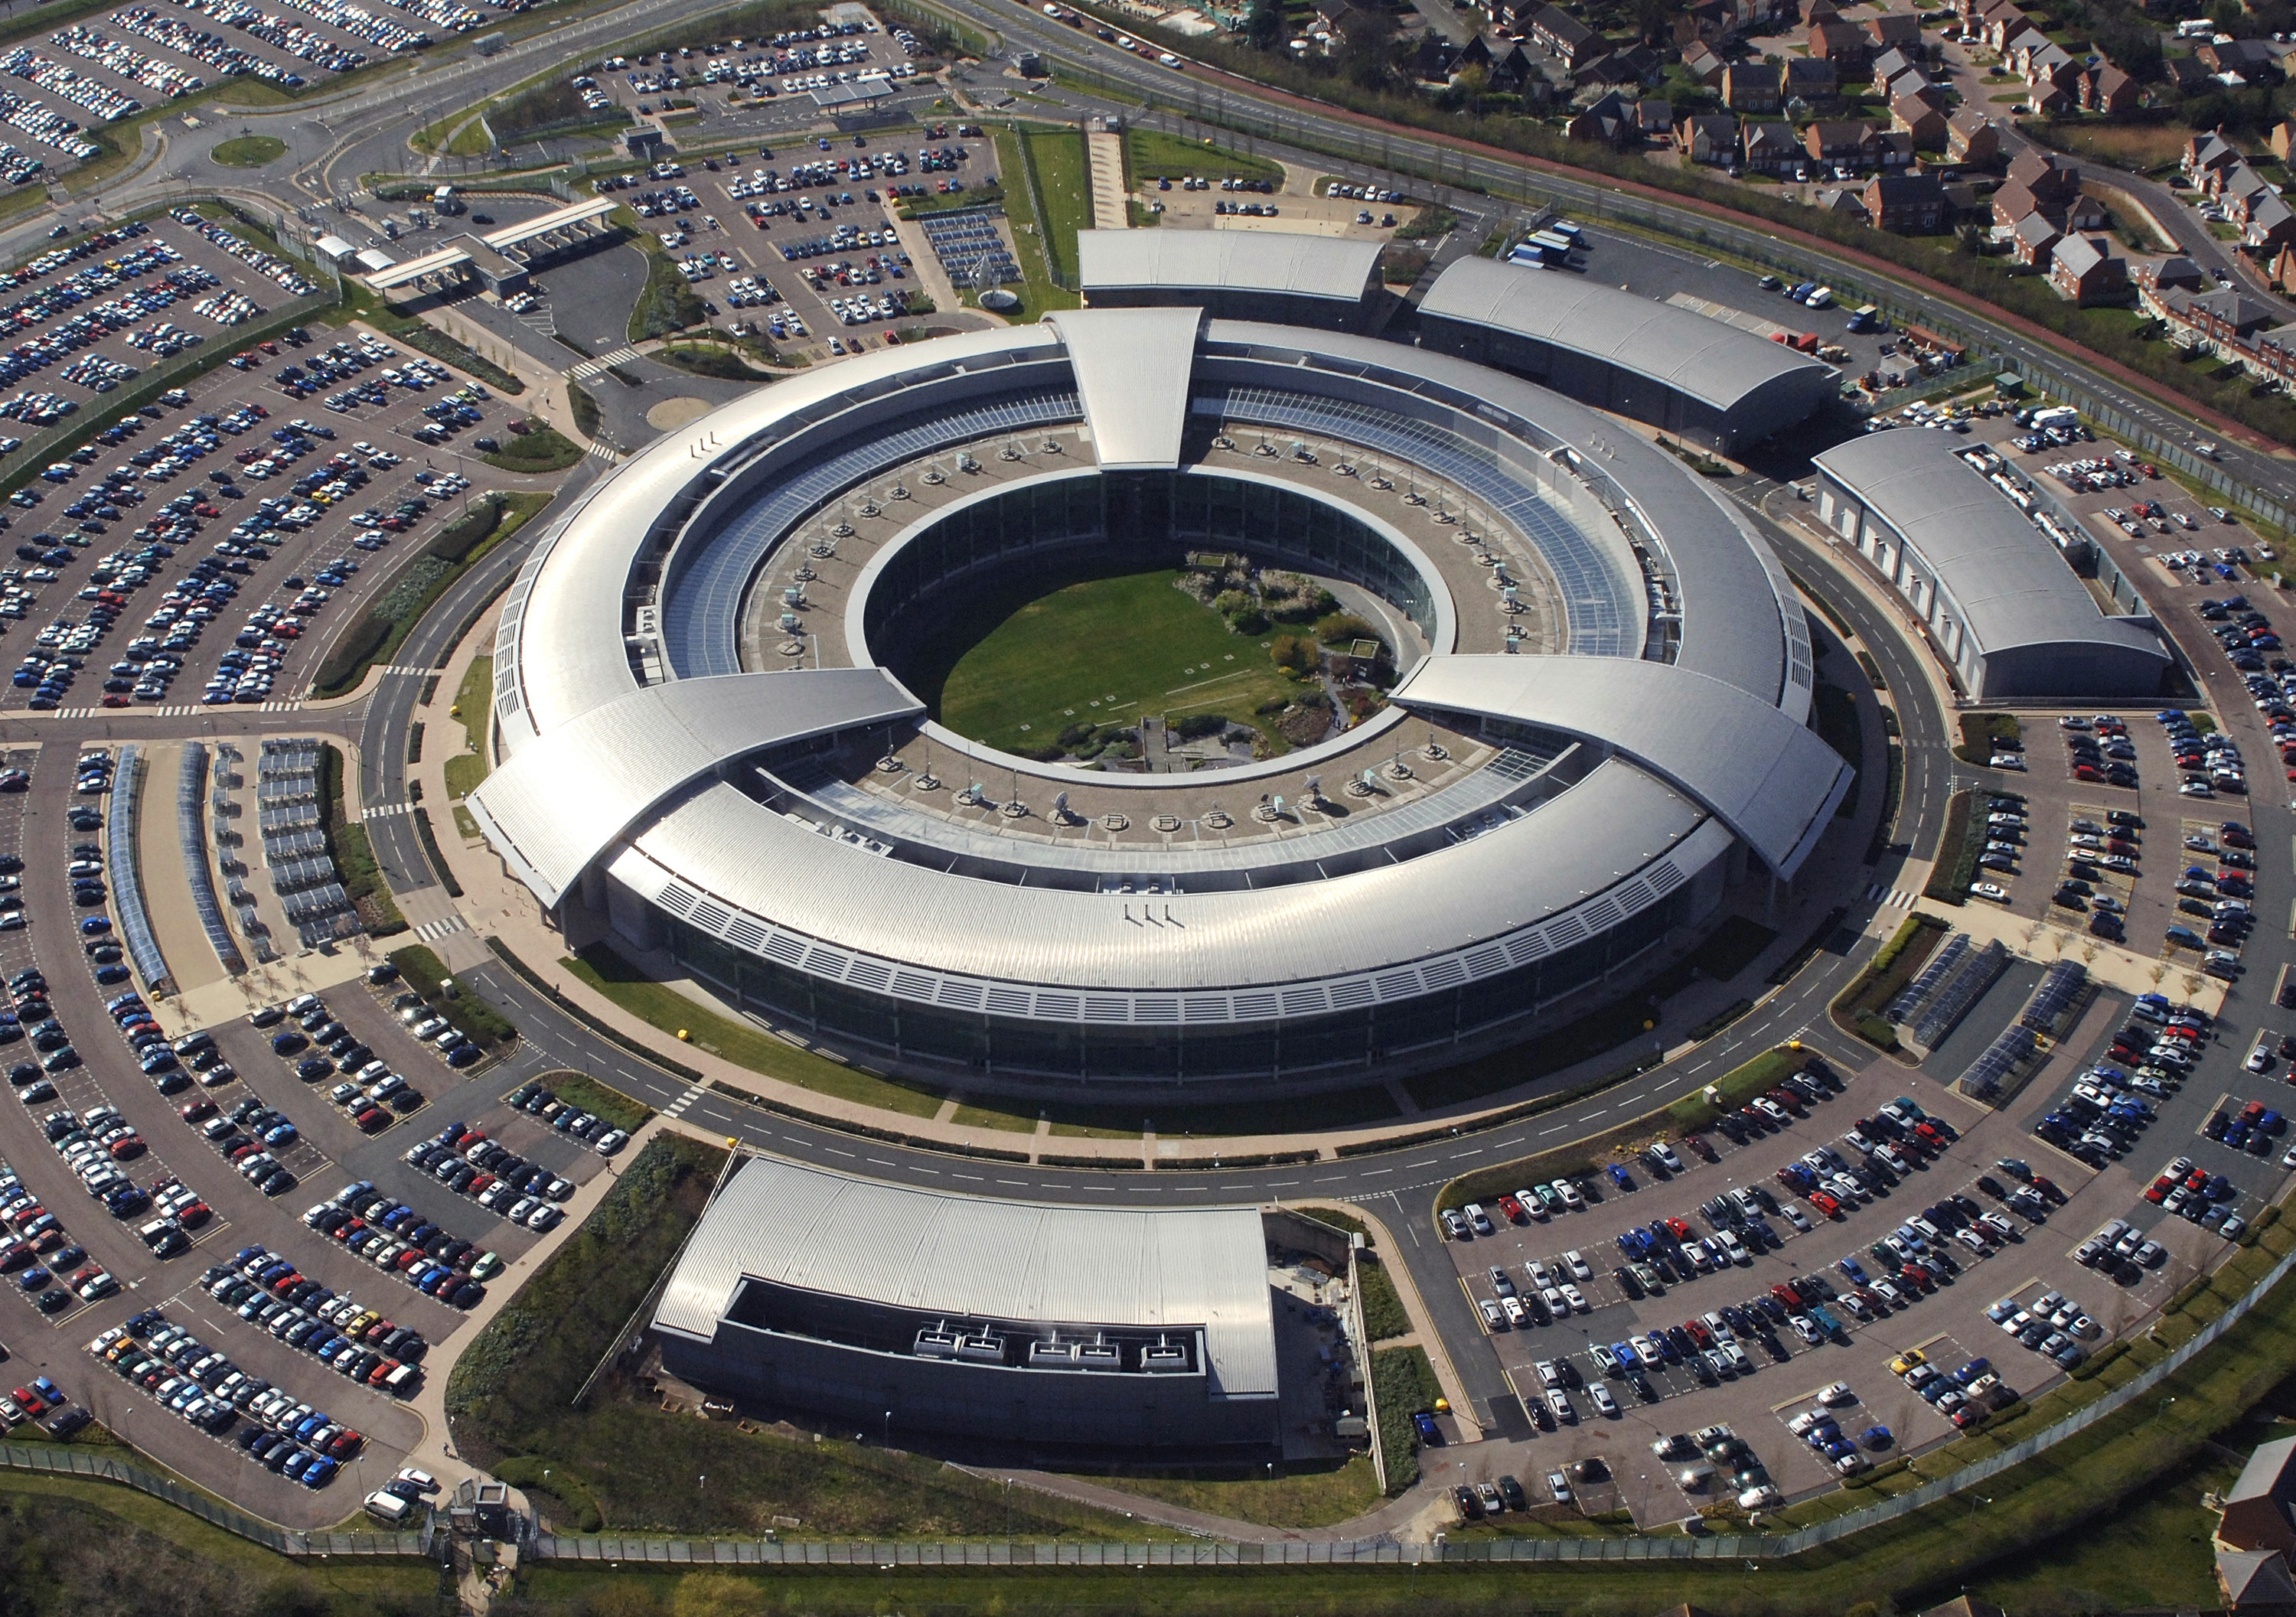
\includegraphics[scale=0.4]{gchq.jpg}
\caption[Les bureaux du GCHQ en photographie aérienne][6pt]{Les bureaux du GCHQ en photographie aérienne.}
\label{fig:gchq}
\end{figure}